\documentclass{article}
\usepackage[utf8]{inputenc}
\usepackage{CJKutf8}
\usepackage[a4paper, margin=0.75in]{geometry}
\usepackage{amsmath,amssymb}
\usepackage{setspace}
\usepackage{graphicx}
\graphicspath{{./images/}}

\setstretch{2}

\begin{document}
\begin{CJK*}{UTF8}{bkai}
    \begin{center}
        {\Huge \textbf{Computer Organization Lab04 Report}}
        {\large \textbf{Author:} 109652039 林立倫, 109550003 陳茂祥}
    \end{center}
\end{CJK*}

\section{Implementation}

\subsection{Decoder}

With the 7-bit input opcode, the decoder will output the corresponding control signals.
We implement the decoder using case statement with opcode as the switch condition.
For don't care signals, we set them to 0.

\subsection{Immediate Generator}

\paragraph{}
With 32-bit instruction as input, 
we can generate the immediate value using concatenation and replication operations as follows:

\begin{center}
    \begin{tabular}{c|c|l}
    opcode & immediate value & Note \\
    \hline
    0110011 & \verb|32'b0| & R-type \\
    0010011 & \verb|{ { 21{ sign } }, instr_i[30:20] }| & ADDI \\
    0000011 & \verb|{ { 21{ sign } }, instr_i[30:20] }| & Load \\   
    0100011 & \verb|{ { 21{ sign } }, instr_i[30:25], instr_i[11:7] }| & Store \\
    1100011 & \verb|{ { 20{ sign } }, instr_i[7], instr_i[30:25], instr_i[11:8], 1'b0 }| & Branch \\
    1101111 & \verb|{ { 12{ sign } }, instr_i[19:12], instr_i[20], instr_i[30:21], 1'b0 }| & JAL \\
    1100111 & \verb|{ { 21{ sign } }, instr_i[30:20] }| & JALR \\
    \end{tabular}
\end{center}

\noindent
where \verb|sign| is the 31st bit of the instruction.

\newpage

\subsection{ALU Control}

\paragraph{}
The ALU control is defined as follows:

\begin{center}
    \begin{tabular}{c|c|c|l}
        ALUOp & instr ($\text{I}_{30}$+func3) & ALU Control & Note                                   \\
        \hline
        00    & -                             & 0010        & Load / Store                           \\
        \hline
        01    & -                             & 0110        & Branch                                 \\
        \hline
              & 0000                          & 0010        & Addition                               \\
              & 1000                          & 0110        & Subtraction                            \\
        10    & 0111                          & 0000        & Bitwise AND                            \\
              & 0110                          & 0001        & Bitwise OR                             \\
              & 0010                          & 0111        & Set on Less Than
    \end{tabular}
\end{center}

\subsection{ALU}

\paragraph{}
The 32-bit ALU is implemented using builtin operators.
Note that SLT instruction depends on the result of addition, 
we choose the result to be \verb|32'b0| or \verb|32'b1| correspond to the 31st bit of the addition result.
In order to determine whether the input \verb|src1| and \verb|src2| need to be inverted or not, 
we use tenary conditional operator to decide the actual operands of the operations. 

\subsection{Simple Single CPU}
Simply connect the wire to the corresponding input and output.
We defined the additional wires as follows:
\begin{figure}[!htb]
    \centering
    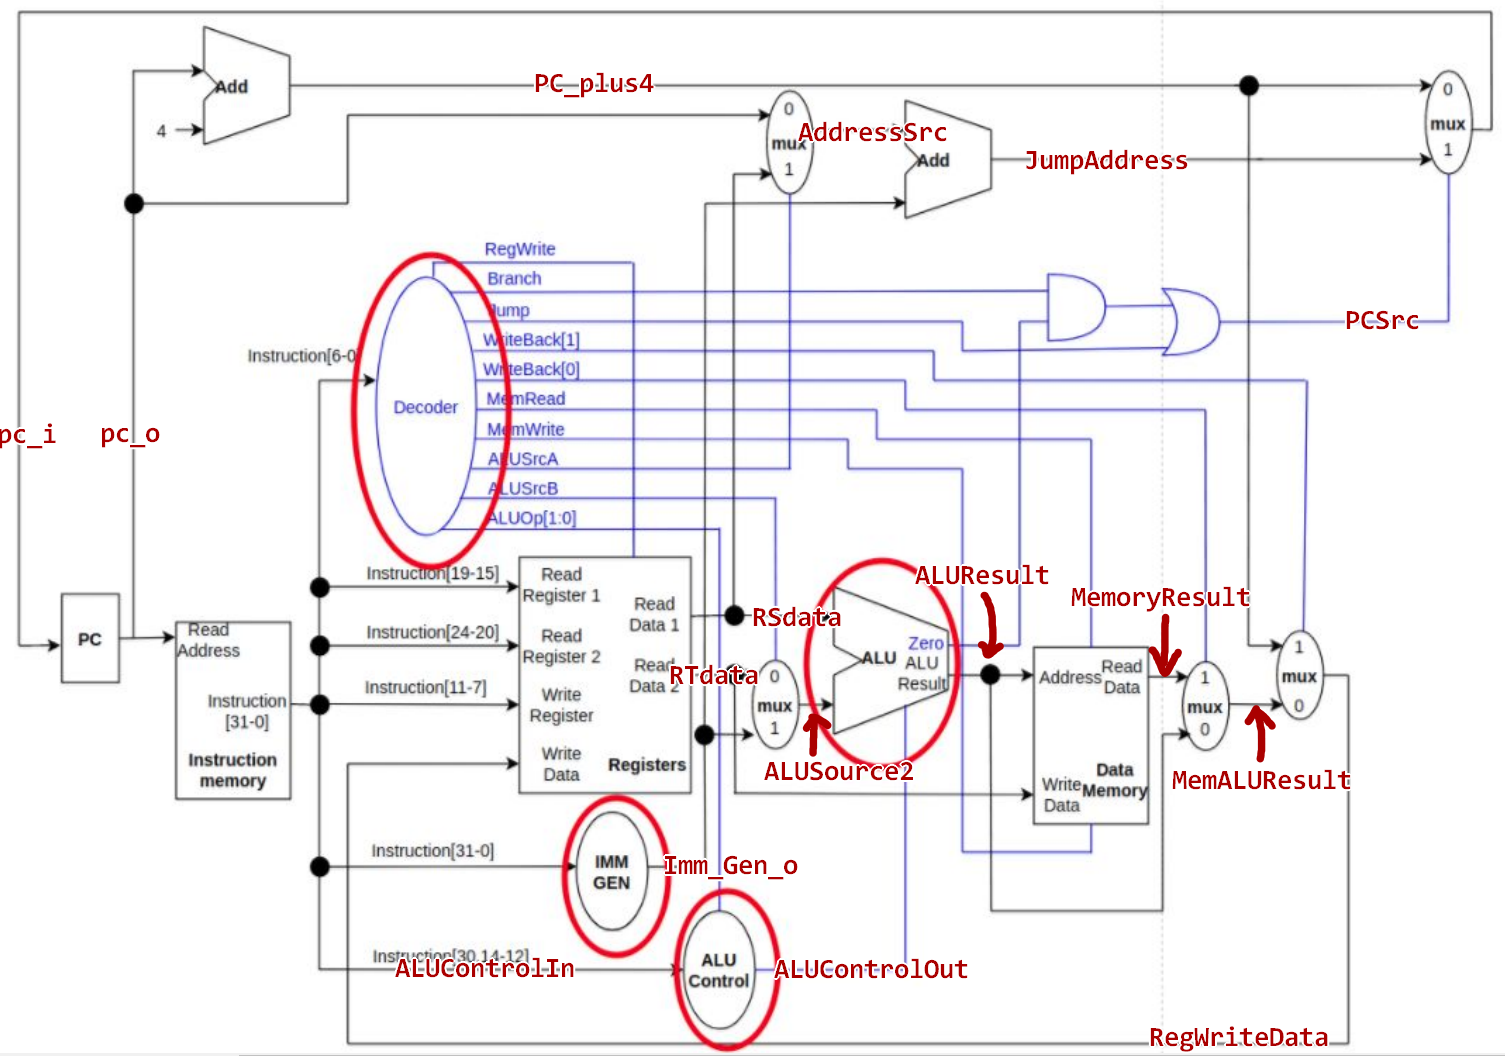
\includegraphics[width=0.75\textwidth]{wire.png}
\end{figure}

\newpage

\section{Result}
\begin{figure}[!htb]
    \centering
    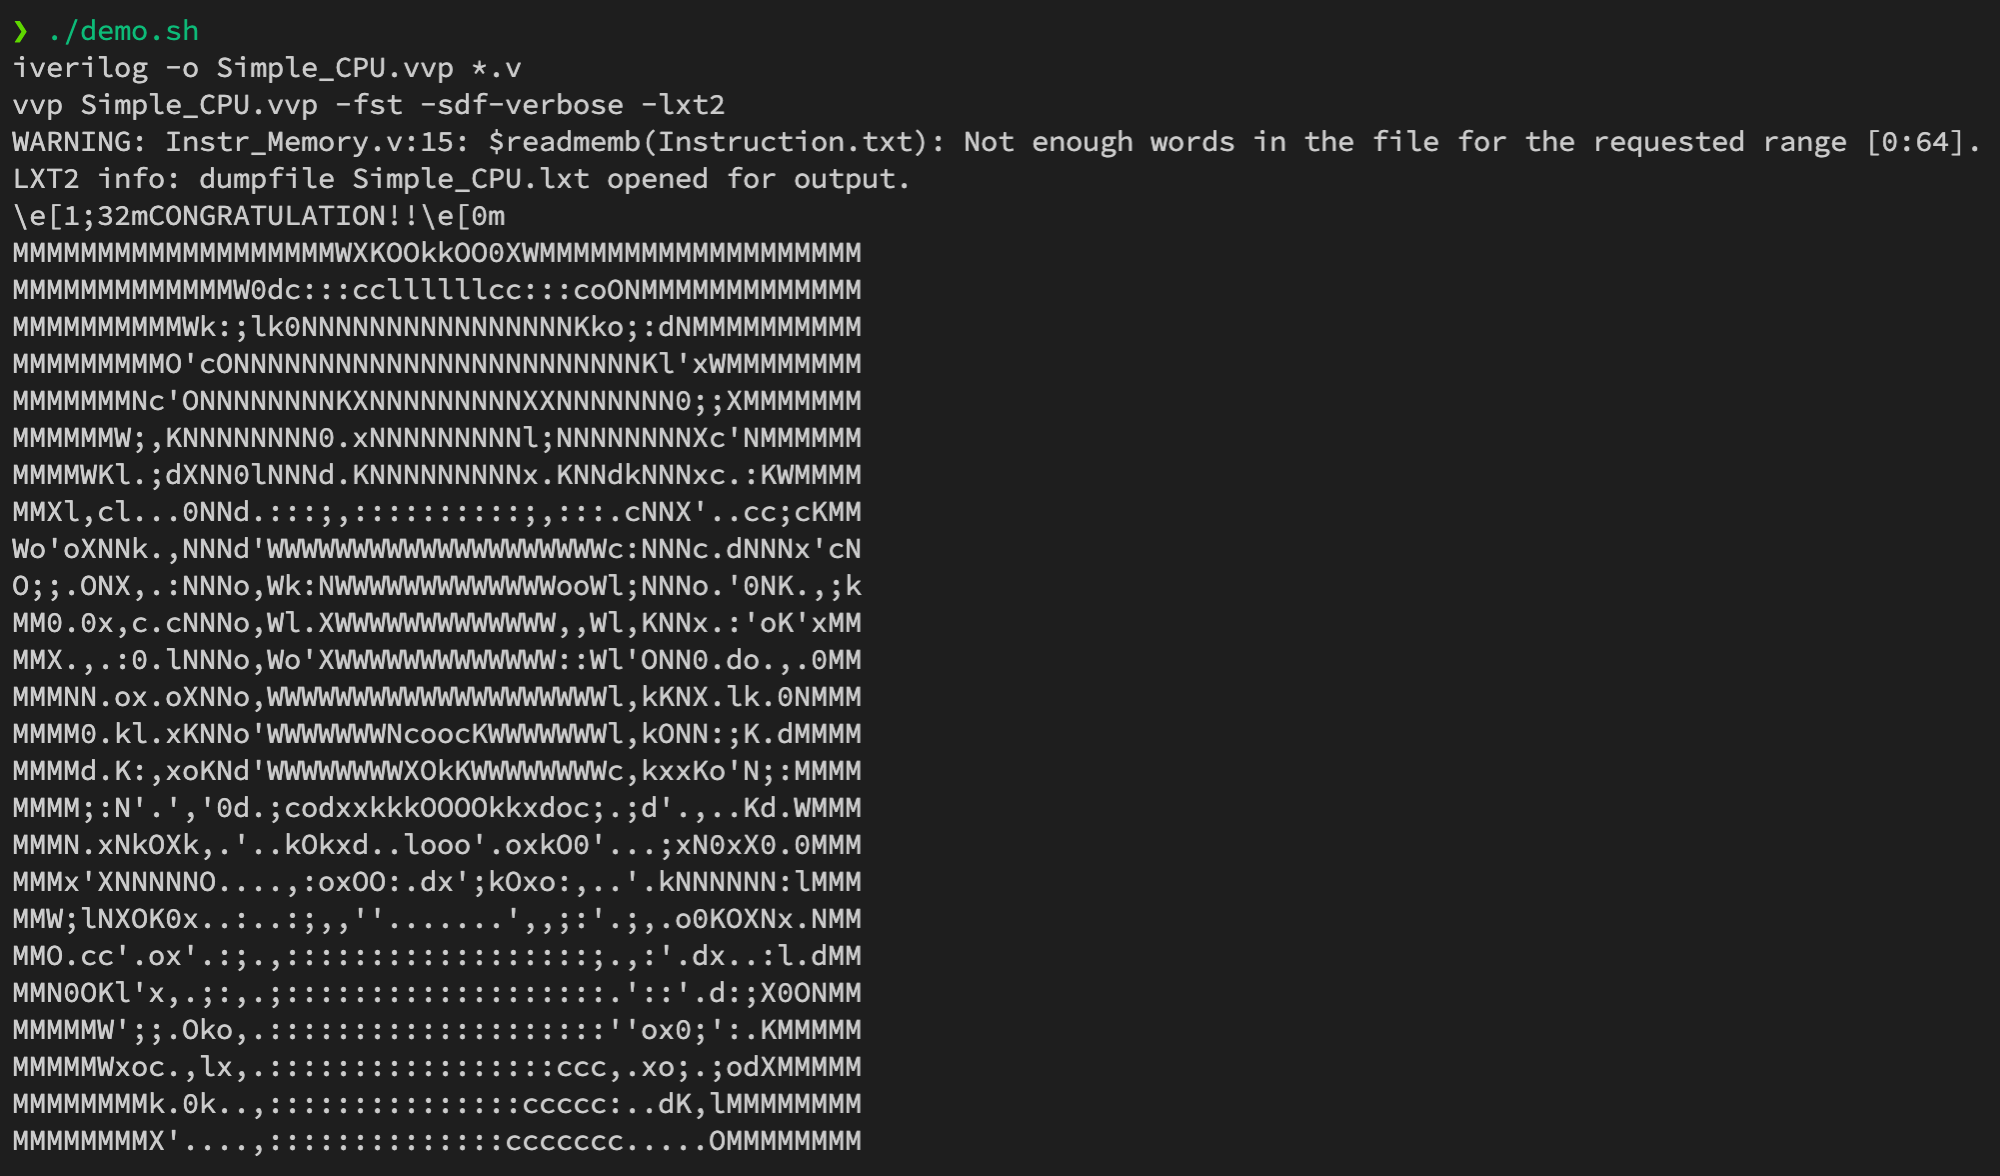
\includegraphics[width=0.75\textwidth]{result.png}
    \caption{Simulation Result}
\end{figure}

\section{Difficulties and Solutions}
\begin{itemize}
    \item The simulation is composed of lots of instructions, therefore it's hard to find bugs on specific instructions.
    \textbf{\textit{Solution:}}  \verb|make| the testbench ourselves,  
     and use the \verb|diff| tool to find the differences in output which contains the information of what the instruction is,
     so that we can add \verb|$display()| to show result in desired code fragment.
\end{itemize} 

\end{document}